\chapter{Evaluation}
\label{chap:evaluation}

The presented map-merging algorithm (chapter~\ref{chap:mergingalgorithm}) has been evaluated on number of demanding robotics datasets. The datasets include data captured by small aerial vehicles (sections~\ref{sec:euroc-dataset}, \ref{sec:aau-dataset}) as well as ground-based robots. The datasets include both widely used benchmark datasets in robotics research as well as data recorded by the author.

Sensors used include stereo rig cameras, active \gls{RGB-D} cameras and laser range finders? This variety of sensors and robots covers many typical multi-robot deployments. All datasets has been captured under real-word conditions, none of them uses simulated data.

The evaluation focuses on properties of the presented pair-wise transformation estimation algorithm for pointclouds (section~\ref{sec:estimate-pair-wise}), which is the core algorithm of the implemented map-merging \gls{ROS} node (section~\ref{sec:ros-package}). Accuracy of the estimation algorithm is critical for the overall map-merging process.

\section{The EuRoC micro aerial vehicle datasets}
\label{sec:euroc-dataset}

The publicly available dataset introduced by~\citet{Burri2016} was collected on-board a micro aerial vehicle (figure~\ref{fig:euroc_platform}) equipped with stereo camera rig and \gls{IMU}. Calibration data for the cameras and ground-truth data are provided with the dataset. This dataset has been used extensively by researches for evaluation of the visual \gls{SLAM} algorithms and visual odometry approaches.

\begin{figure}
    \centering
    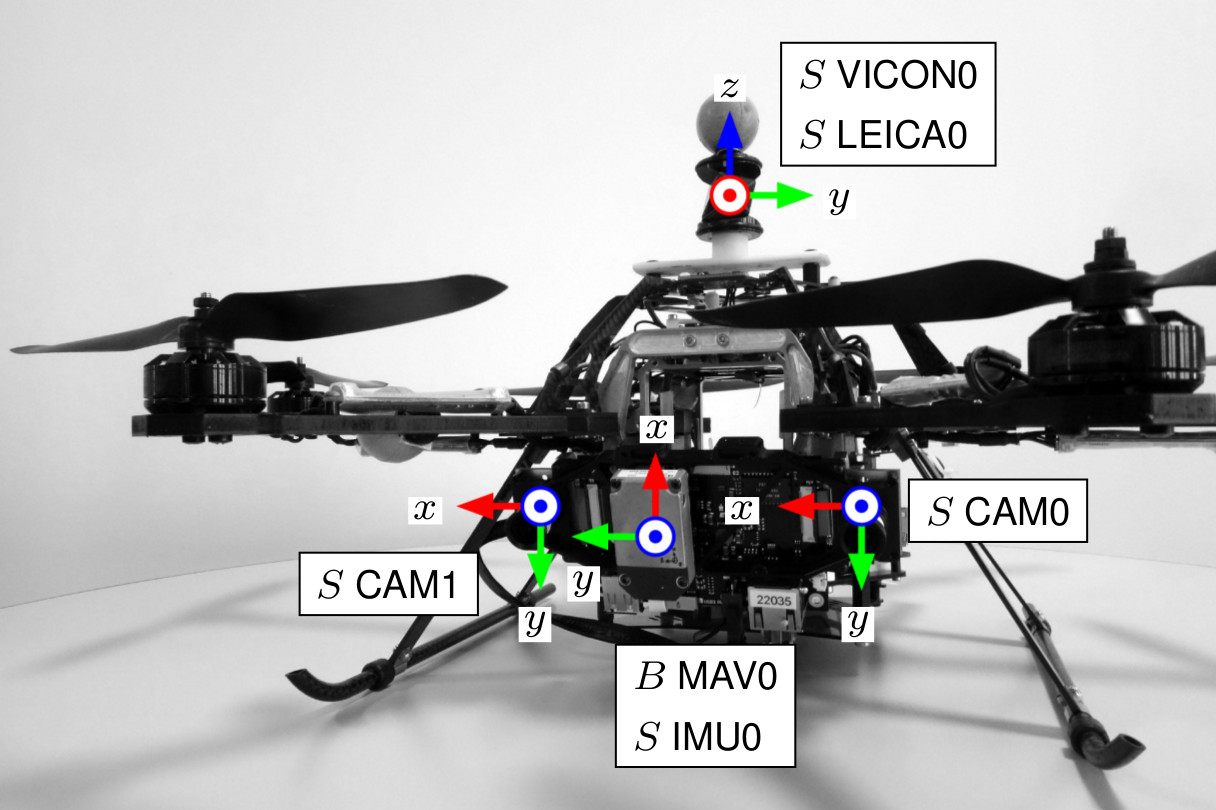
\includegraphics[width=\textwidth]{../img/euroc_platform.jpg}
    \caption[A micro aerial vehicle]{An Asctec Firefly hex-rotor micro aerial vehicle used for collecting the EuRoC micro aerial vehicle datasets. The picture shows reference frames of the sensors -- the stereo cameras and \gls{IMU}.}
    \label{fig:euroc_platform}
\end{figure}

\subsection{Dataset description}

The cameras produce a WVGA monochrome (greyscale) images at $20$ frames per second. Cameras have a global shutter. The automatic exposure control is independent for both cameras. According to the published errata~\citep{Burri2016}, this resulted in different shutter times and in turn in different image brightnesses, rendering stereo matching and feature tracking more challenging.

The dataset contains $11$ mapping sessions in $3$ different environments (``Machine Hall'', ``Vicon Room 1'', ``Vicon Room 2''). Each mapping session is available in a single \gls{ROS} bag file. First $5$ sessions were captured in ETH machine hall (figure~\ref{fig:eth-machine-hall}), a fairly large industrial environment featuring piping, reservoirs and many different types of surfaces. Second and third batch of datasets were captured in a smaller furnished rectangular room. For the second and the third batch the furnishing was different.

\begin{figure}
    \centering
    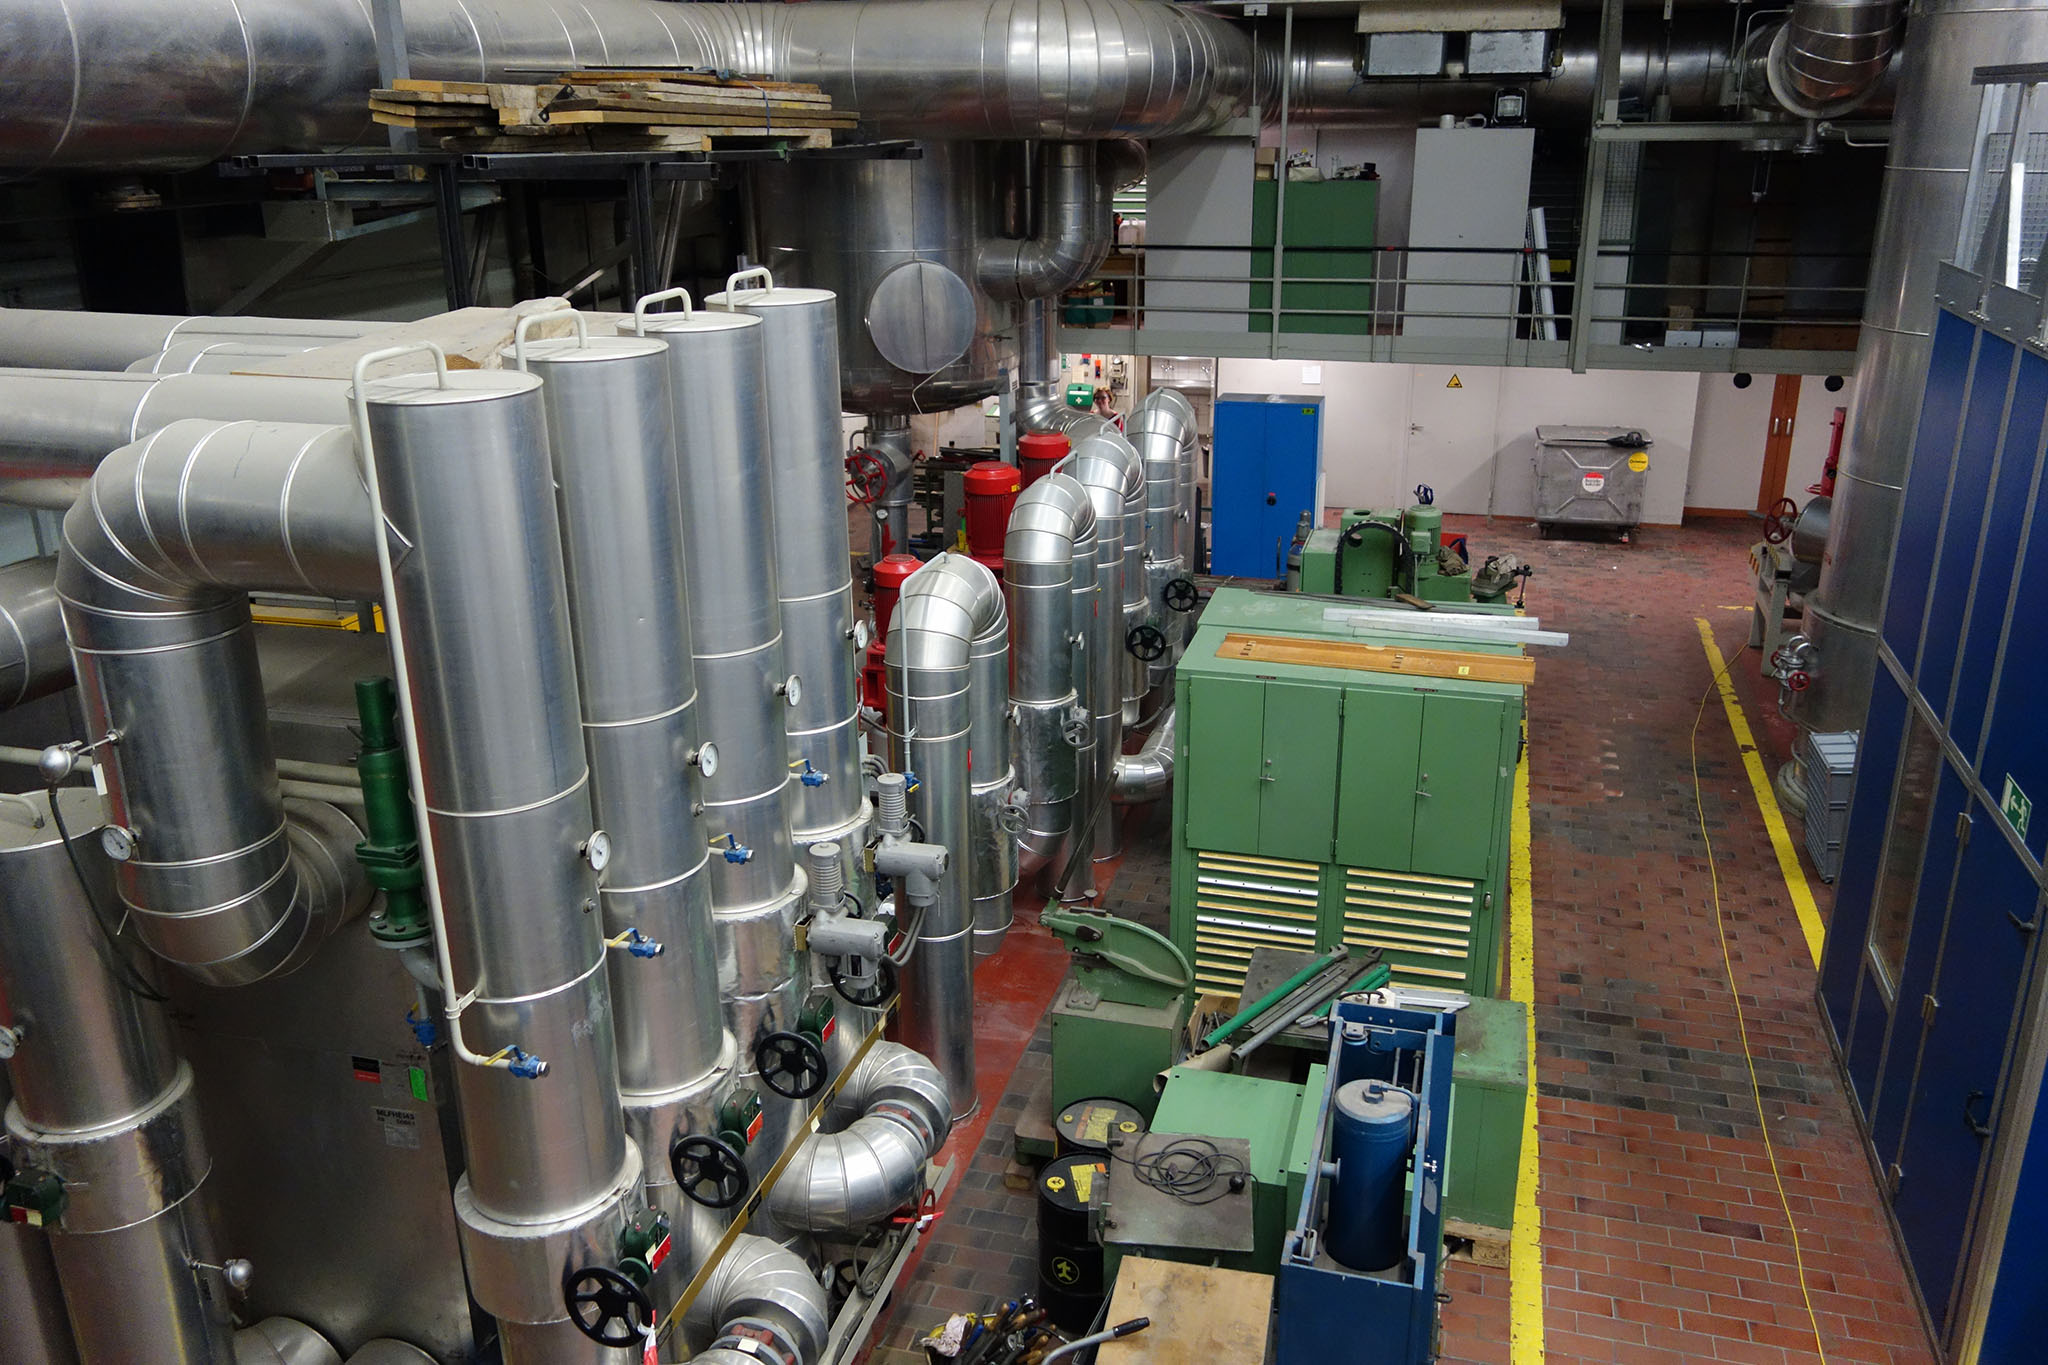
\includegraphics[width=\textwidth]{../img/eth_machine_room.jpg}
    \caption[ETH Machine hall]{ETH Machine hall industrial environment where $5$ mapping sessions of EuRoC dataset were captured. The image is courtesy of the authors~\citep{Burri2016}.}
    \label{fig:eth-machine-hall}
\end{figure}

\subsection{Maps generation}
\label{sec:euroc-generating-maps}

The dataset is intended for evaluating \gls{SLAM} algorithms, for our purposes it was necessary to process the data with a \gls{SLAM} algorithm to create a pointcloud maps.

First, I have used the provided calibration sequence and I have created a calibration data for \gls{ROS} using the \texttt{camera\_calibration} tool available with \gls{ROS}.

Second, for each environment I created a pair of maps using the $01$ and $02$ mapping sessions from the datasets, which were used further for the evaluation of the map-merging (figures~\ref{fig:euroc_mh_02}, \ref{fig:v1-greyscale}, \ref{fig:euroc_v2_02}). I used a RTAB-Map \gls{SLAM}, developed by~\citet{labbe2014online}, to create the maps. The odometry for mapping was provided from stereo camera data, using a visual odometry approach, the available \gls{IMU} data were not used. For the $01$ sessions I have used a native visual odometry approach of RTAB-Map. For the $02$ sessions I have used visual odometry approach of {ORB-SLAM2}, introduced by~\citet{mur2017orb}, because the data exhibit more dynamic motions, which lead to frequent loss on visual odometry using the first approach. {ORB-SLAM2} visual odometry exhibited better robustness for this data. In both cases loop-closure approach of~\citet{labbe2014online} has been used.

The maps has been voxelised to the resolution of $0.05$ meter per voxel, which yields suitable map sizes for map exchange in a multi-robot system.

Using a different \gls{SLAM} pipelines for each of the maps contributed to introducing different mapping errors and artefacts, which makes map-merging of such maps more difficult.

\begin{figure}
    \centering
    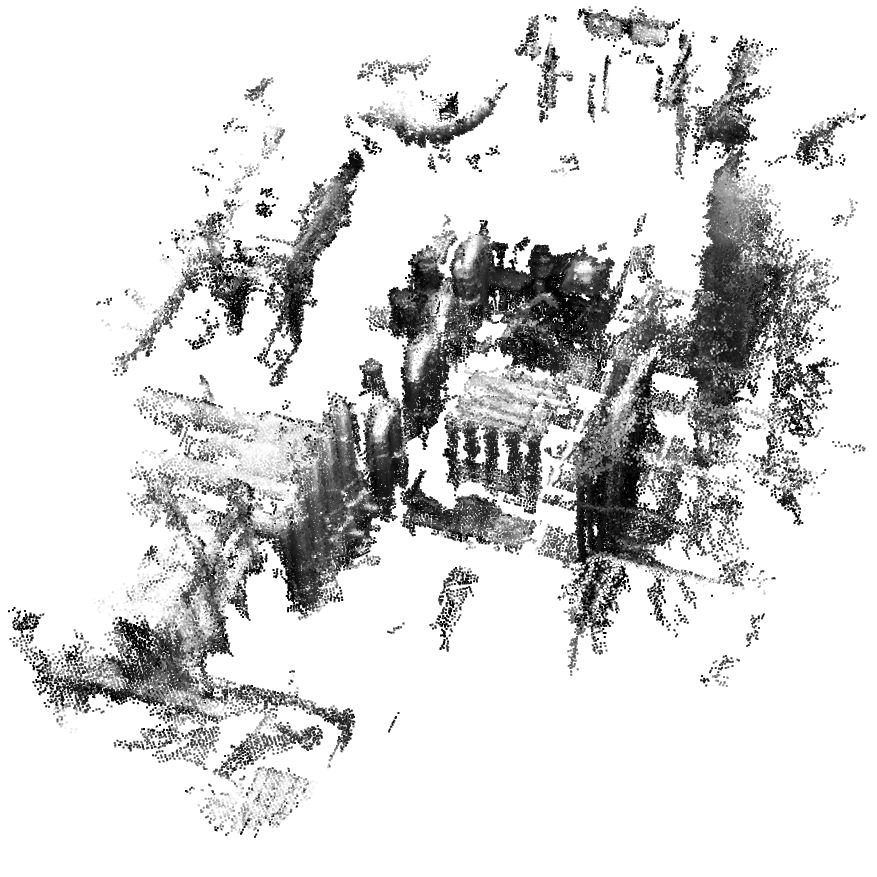
\includegraphics[width=\textwidth]{../img/euroc_mh_02.png}
    \caption[Machine hall pointcloud map]{ETH Machine hall pointcloud map. The map was produced from ``Machine Hall 02'' dataset using an {ORB-SLAM2} visual odometry~\citep{mur2017orb} and RTAB-Map loop-closure approach~\citep{labbe2014online}.}
    \label{fig:euroc_mh_02}
\end{figure}

\begin{figure}
    \centering
    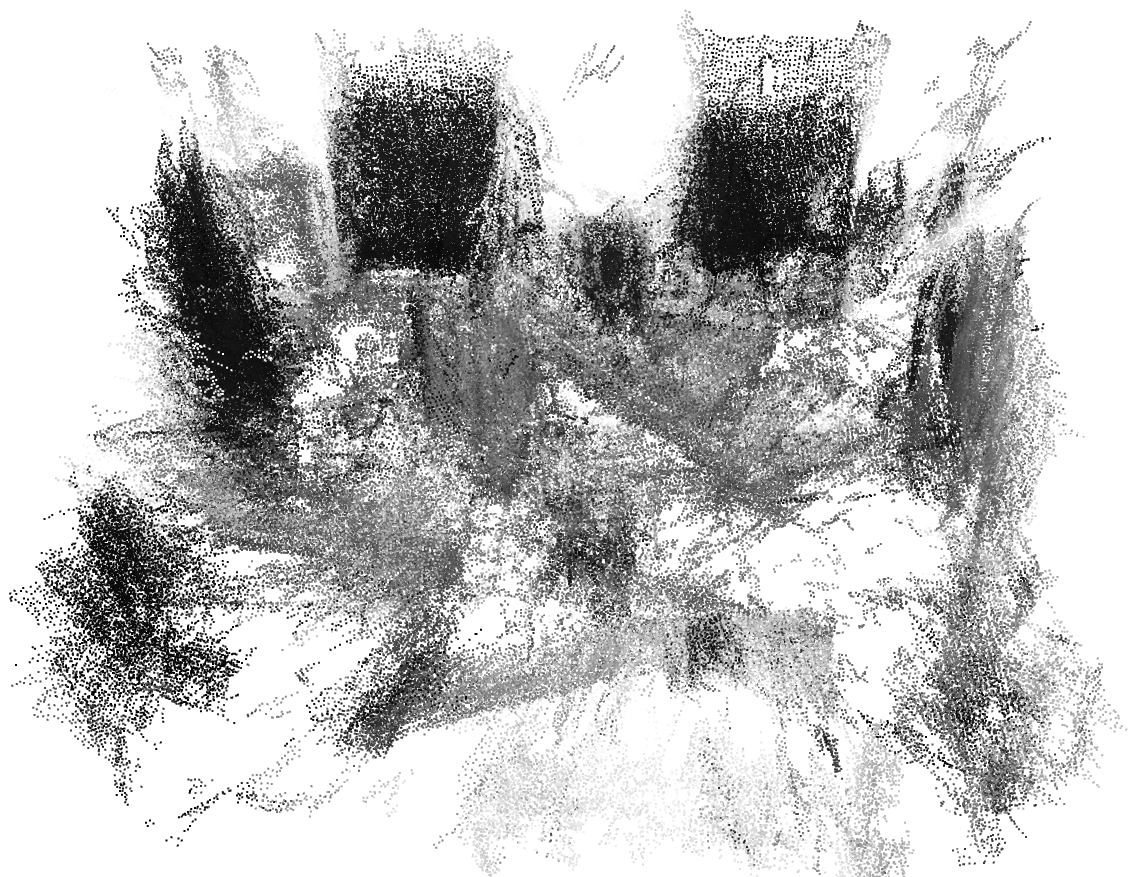
\includegraphics[width=\textwidth]{../img/euroc_v2_02.png}
    \caption[Pointcloud map of a small room]{A pointcloud map of a small room. The map was produced from ``Vicon Room 2 02'' dataset using an {ORB-SLAM2} visual odometry~\citep{mur2017orb} and RTAB-Map loop-closure approach~\citep{labbe2014online}.}
    \label{fig:euroc_v2_02}
\end{figure}

\section{AAU dataset}
\label{sec:aau-dataset}

The dataset recorded at \acrfull{AAU} on-board a micro aerial vehicle in an outdoor forest environment. The vehicle was equipped with a stereo camera rig and \gls{IMU}. The cameras produce greyscale images.

This dataset contains two mapping sessions. The environment consists or medium-sized trees, the ground is covered with leaves. The lighting conditions are challenging as there are areas of direct sunlight as well as areas in the shade. The lighting conditions are similar in the both sessions, as the sessions were captured in the similar time of day. This setup causes difficult conditions for stereo matching and pose estimation, introducing mapping errors into the maps, which in turn make the map-merging a challenging task.

Maps (figures~\ref{fig:aau_top}, \ref{fig:aau_lateral}) were generated in the similar manner as described in section~\ref{sec:euroc-generating-maps}. Mapping has been done with RTAB-Map \gls{SLAM}~\citep{labbe2014online} using a its native visual odometry approach.

% todo atribution

\begin{figure}
    \centering
    \begin{subfigure}[b]{0.82\textwidth}
        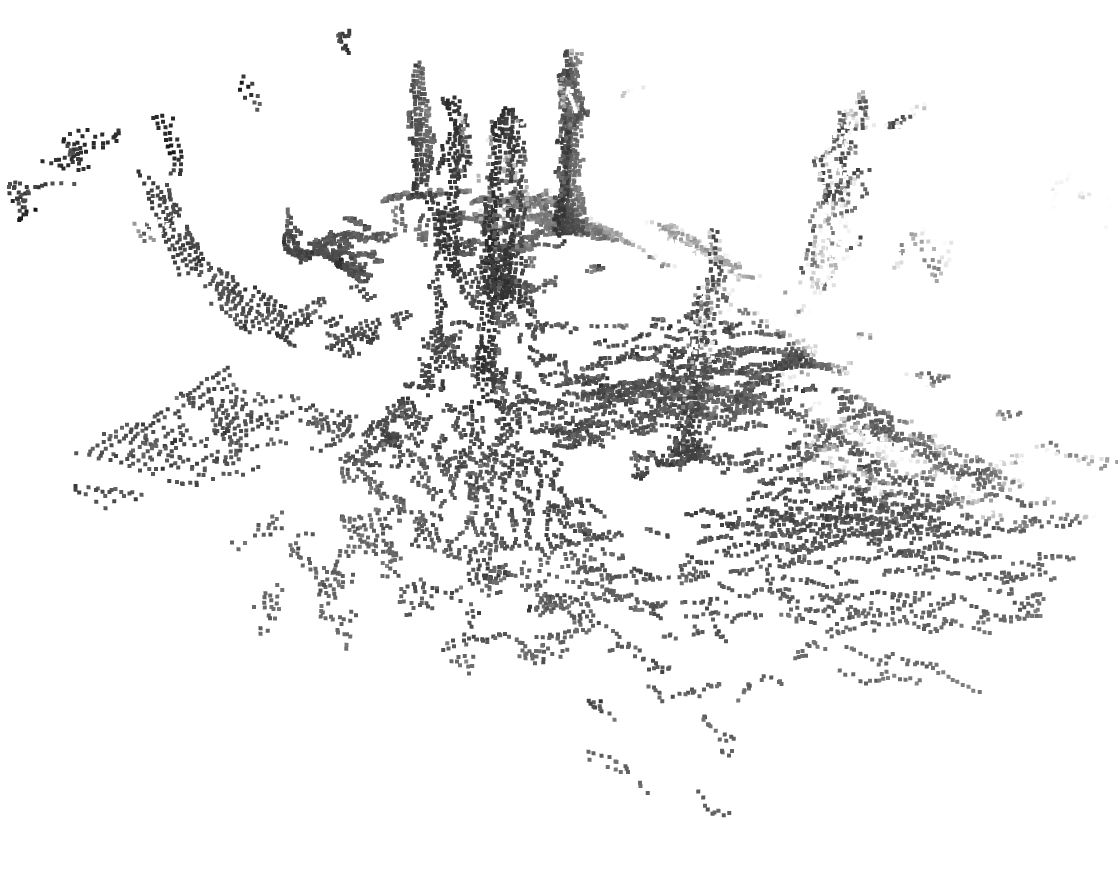
\includegraphics[width=\textwidth]{../img/aau_fc_dnav5_top.png}
        \caption{``\gls{AAU} forest 1'' map}
    \end{subfigure}
    % ~
    \begin{subfigure}[b]{0.82\textwidth}
        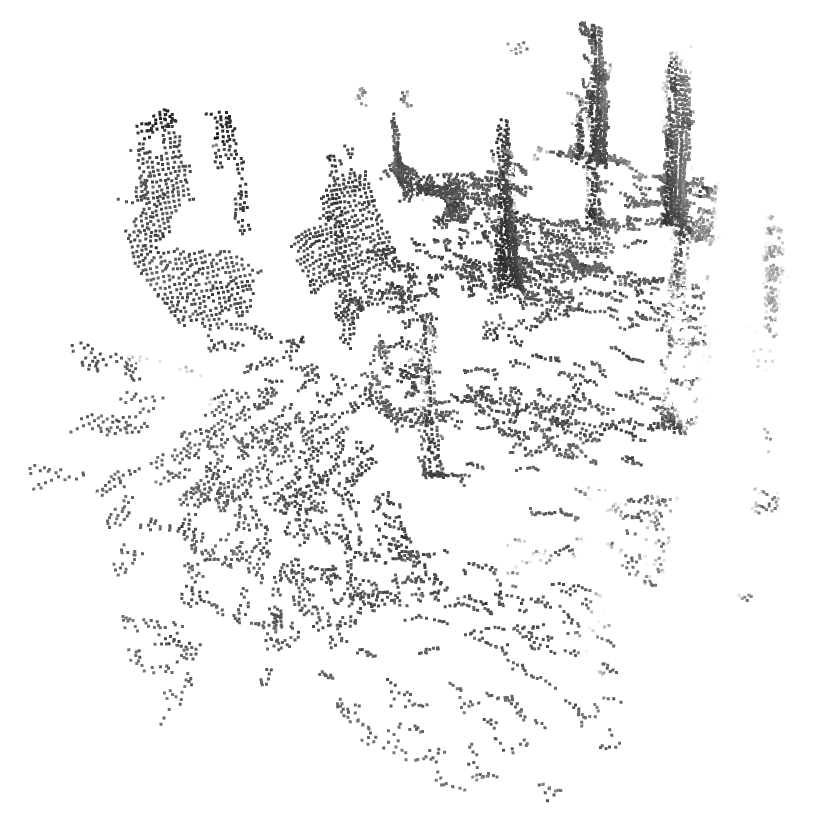
\includegraphics[width=\textwidth]{../img/aau_fc_dnav6_top.png}
        \caption{``\gls{AAU} forest 2'' map}
    \end{subfigure}
    \caption[Forest pointcloud maps -- top view]{Top view of the two pointcloud maps from \gls{AAU} outdoor forest dataset. Notice the stripe of direct sunlight on the ground causing difficult conditions for stereo matching.}
    \label{fig:aau_top}
\end{figure}

\begin{figure}
    \centering
    \begin{subfigure}[b]{\textwidth}
        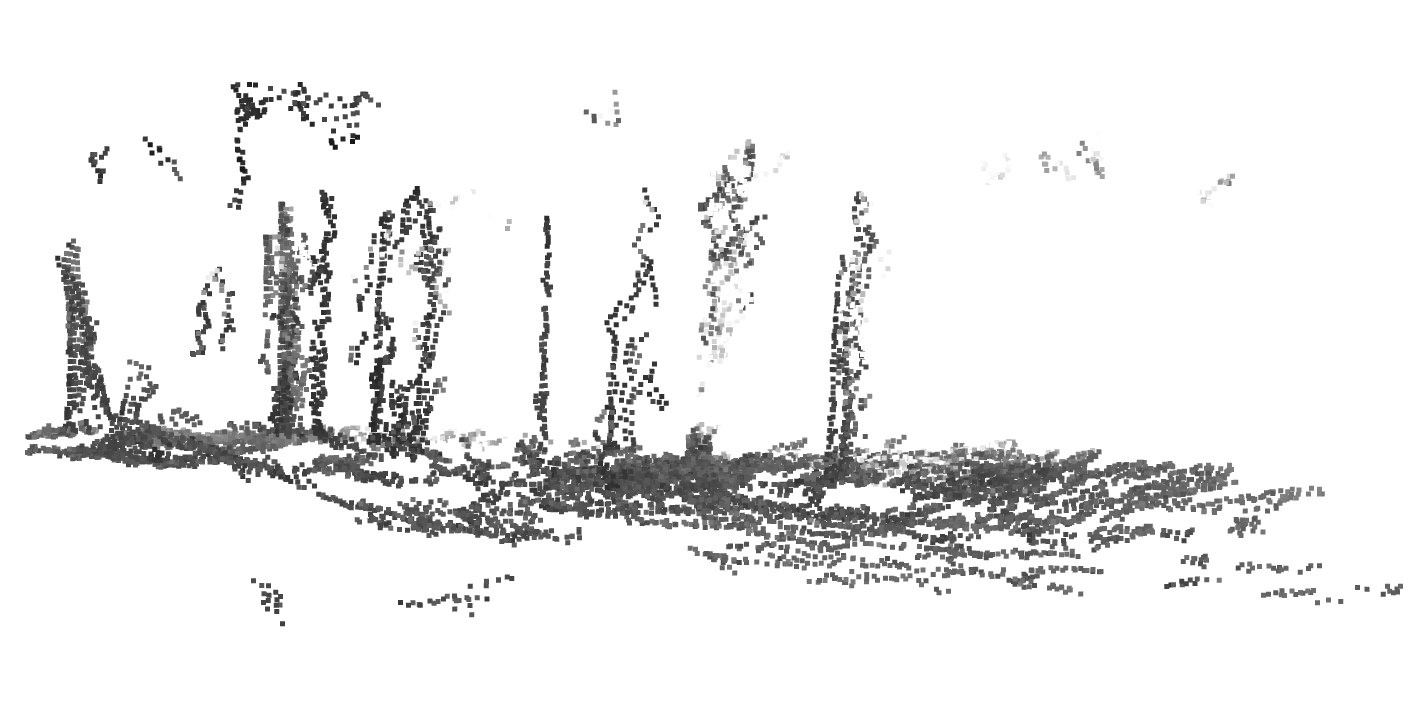
\includegraphics[width=\textwidth]{../img/aau_fc_dnav5_lateral.png}
        \caption{``\gls{AAU} forest 1'' map}
    \end{subfigure}
    % ~
    \begin{subfigure}[b]{\textwidth}
        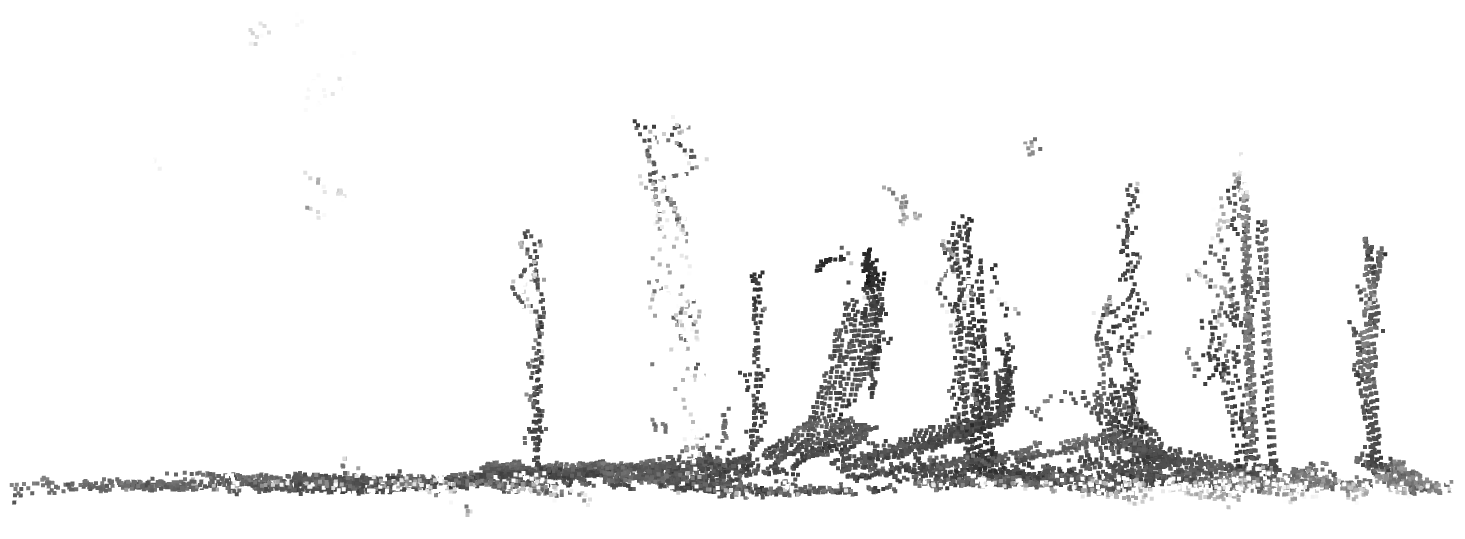
\includegraphics[width=\textwidth]{../img/aau_fc_dnav6_lateral.png}
        \caption{``\gls{AAU} forest 2'' map}
    \end{subfigure}
    \caption[Forest pointcloud maps -- lateral view]{Lateral view of the two pointcloud maps from \gls{AAU} outdoor forest dataset. In both maps there is a non-flat terrain and number of outliers caused by branches and difficult mapping conditions.}
    \label{fig:aau_lateral}
\end{figure}

\section{MFF dataset}
\label{sec:mff-dataset}